\chapter{Inleiding}

Op dit eigenste moment zijn er waarschijnlijk enkele honderden \emph{spiders} actief op internet.
Die computerprogramma's, die soms ook \emph{robots} of \emph{wanderers} worden genoemd, reizen
het internet rond om bepaalde documenten -- in het bijzonder beelden -- te localiseren. Ze indexeren
de gevonden documenten in een databank, die dan doorzocht kan worden door een zoekmachine. 

Zoekmachines zoals \emph{Google} en \emph{Yahoo} hebben op die manier reeds databanken
opgebouwd die meer dan een miljard beelden bevatten. Het wordt bijgevolg steeds belangrijker
om manieren te zoeken om die gigantische collecties van beelden op een effici\"ente wijze
te doorzoeken.


\section{Tekstgebaseerd zoeken van beelden}

Alle belangrijke bestaande zoekmachines bieden \emph{text-based image retrieval} (TBIR) aan. 
Figuur~\ref{fig:tbir} toont de algemene architectuur van die machines. Elk beeld 
wordt voorzien van tekstuele annotaties, zoals bijvoorbeeld de 
bestandsnaam of woorden uit de webpagina waarvan het deel uitmaakt. Die annotaties
worden gebruikt voor het indexeren van de beelden in de databank.

De gebruiker van een TBIR-systeem start een zoekactie door \'e\'en of meerdere trefwoorden door te geven
aan het systeem. Het systeem vergelijkt die trefwoorden vervolgens met de annotaties uit
de databank. De beelden waarvan er annotaties overeenkomen met een trefwoord, maken
deel uit van het resultaat van de query. Daarvoor is het uiteraard niet nodig om alle beelden
uit de databank te overlopen, vermits de databank ge\"indexeerd is op de annotaties. 

\section{Inhoudgebaseerd zoeken van beelden}

Omdat de tekstgebaseerde aanpak in de praktijk dikwijls tekortschiet, is men op zoek gegaan 
naar manieren om het zoeken te baseren op de visuele inhoud van de beelden 
\cite{smeulders:cbir_end_of_early_years}. Zo zijn de \emph{content-based image retrieval} (CBIR) systemen 
\cite{veltcamp:cbirs} ontstaan. 
De algemene architectuur van een dergelijk systeem wordt ge\"illustreerd door
figuur~\ref{fig:cbir}. Er wordt gebruik gemaakt van een proces dat \emph{kenmerkextractie}
(\emph{(visual) feature extraction}) genoemd wordt \cite{rui:image_retr}. Dat proces zet een beeld om in een 
\emph{kenmerkvector} (\emph{feature vector}). Met behulp van multidimensionale indexering kan die
vector dan gebruikt worden als alternatief voor de tekstuele annotaties bij TBIR.

De meeste CBIR-systemen werken volgens het \emph{query-by-example} principe. Dat houdt in dat de
gebruiker een beeld als voorbeeld opgeeft, waarna het systeem op zoek gaat naar beelden
die visuele gelijkenissen vertonen met dat voorbeeld. Daartoe wordt eerst de kenmerkvector van
het opgegeven beeld bepaald, om deze vervolgens te vergelijken met de kenmerkvectoren in
de databank. Het uiteindelijke resultaat bestaat uit de beelden uit de databank 
waarvan de overeenkomstige vectoren grote similariteit vertonen met de vector van het 
voorbeeld. Doordat de databank ge\"indexeerd is op de kenmerkvectoren, is het niet nodig
om ze volledig te overlopen.

\begin{figure}[tb]
\begin{center}
\subfigure[]{
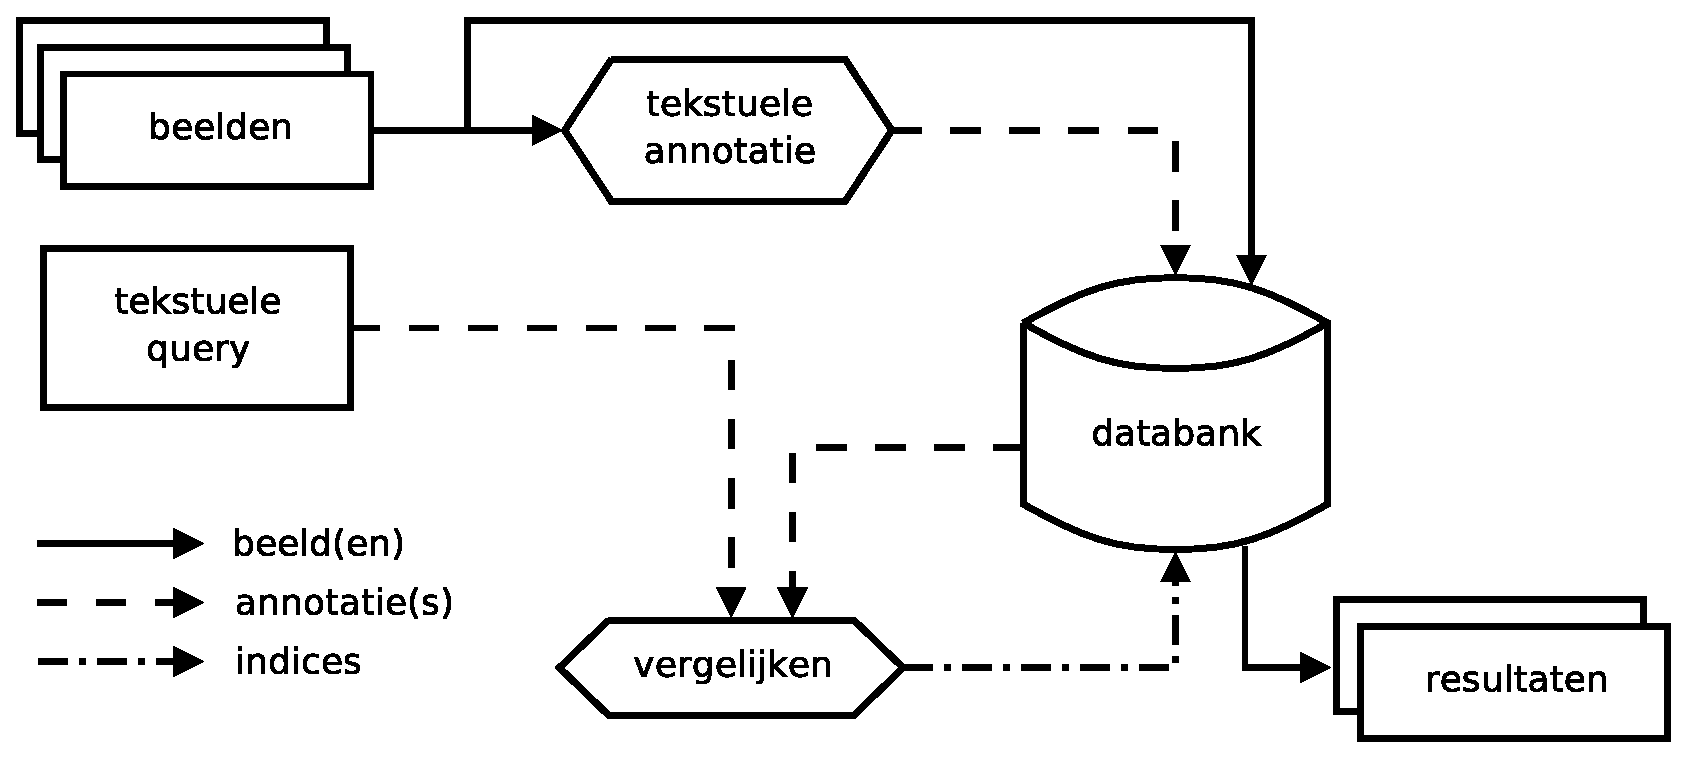
\includegraphics[width=10cm]{images/tbir.eps}
\label{fig:tbir}
}
\vspace{5pt}
\subfigure[]{
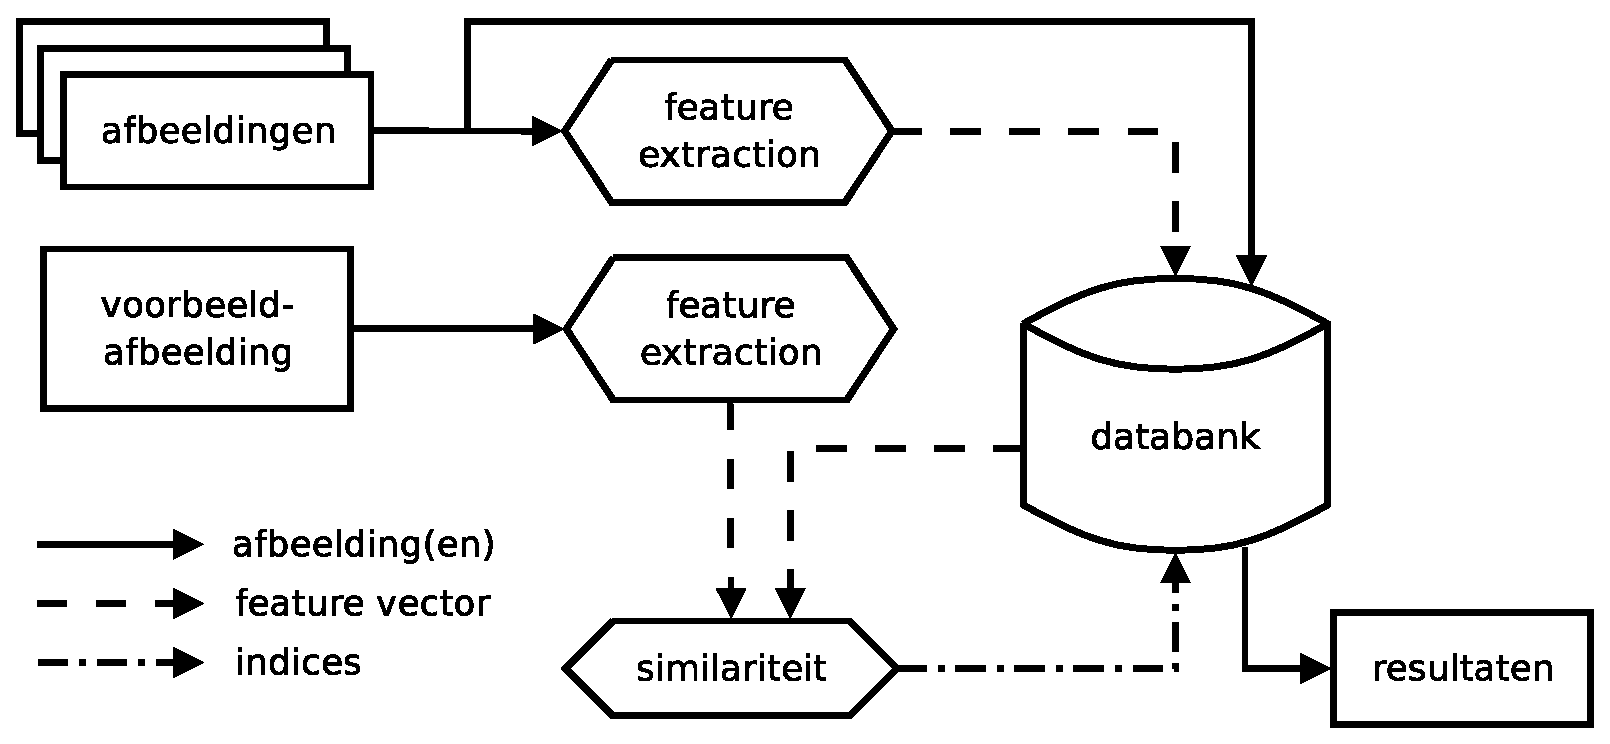
\includegraphics[width=10cm]{images/cbir.eps}
\label{fig:cbir}
}
\caption{\label{fig:cbir_en_tbir}Algemene architectuur van (a) een TBIR- en 
(b) een CBIR-systeem.}
\end{center}
\end{figure}

\section{Similariteitsgebaseerd rangschikken van de zoekresultaten}

Doordat CBIR-systemen zeer complex zijn, is het op dit moment nog niet mogelijk om ze te gebruiken voor het 
doorzoeken van zeer omvangrijke databanken. Bovendien beschikt de gebruiker niet altijd over
een geschikt voorbeeld. Dat probleem kan eventueel nog opgelost worden door gebruik
te maken van een voorbeeld-schets, maar ook dat is in de praktijk niet altijd even handig.

Het is dus zinvol om te zoeken naar manieren om inhoudgebaseerde aspecten toe te voegen aan
TBIR-systemen. De manier die we in deze scriptie bespreken, is het 
similariteitsgebaseerd rangschikken van de resultaten van een TBIR-systeem. Hierbij verwachten we
nog steeds dat de gebruiker een tekstuele query opgeeft, waarop het systeem antwoordt met een 
lijst van beelden die overeenkomen met die query. Daarna heeft de gebruiker echter ook nog 
de mogelijkheid om een verzameling van voorbeelden te kiezen uit die lijst. Het 
systeem zorgt er vervolgens voor dat de zoekresultaten gerangschikt worden in 
volgorde van similariteit met de voorbeelden.

